\documentclass[a4paper,12pt]{report}

% Pakete einbinden
\usepackage[utf8]{inputenc}
\usepackage[T1]{fontenc}
\usepackage{lipsum} % für Lorem Ipsum Beispieltext
\usepackage{graphicx} % für Bilder
\usepackage[backend=biber]{biblatex} % für Zitate und Literaturverzeichnis
\addbibresource{bibliography.bib}

\usepackage{minted}
\usepackage[minted]{tcolorbox}


% Custom JavaScript code box with black border
\newtcblisting{code}{
	listing engine=minted,
	listing only,
	minted language=javascript,
	minted style=colorful,
	minted options={
		linenos,
		fontsize=\small,
		breaklines,
		tabsize=2,
		bgcolor=lightgray!25,
	},
	boxrule=0pt,
	top=0pt, bottom=0pt, left=2pt, right=2pt,
	colback=lightgray!25,
}

% Custom css code box with black border
\newtcblisting{csscode}{
	listing engine=minted,
	listing only,
	minted language=css,
	minted style=colorful,
	minted options={
		linenos,
		fontsize=\small,
		breaklines,
		tabsize=2,
		bgcolor=lightgray!25,
	},
	boxrule=0pt,
	top=0pt, bottom=0pt, left=2pt, right=2pt,
	colback=lightgray!25,
}

% Dokumentenbeginn
\begin{document}

% Titelblatt
\title{Titel der Diplomarbeit}
\author{Dein Name}
\date{\today}
\maketitle

% Abstract
\chapter*{Abstract}
\addcontentsline{toc}{chapter}{Abstract}
\lipsum[1]
\newpage

% Abstract
\chapter*{Kurzfassung}
\addcontentsline{toc}{chapter}{Kurzfassung}
\lipsum[1]
\newpage

% Inhaltsverzeichnis
\tableofcontents
\newpage

% Einleitung
\chapter{Introduction}
Link Gliederung: https://www.diplomarbeiten-bbs.at/durchfuehrung/gliederung-der-diplomarbeit-und-formale-vorgaben
\section{Short description}

The topic of this diploma thesis is creating a platform which supports different voting options like single, multiple or weighted choice. Additionally there should be a Login system with different roles to administer and create or delete polls and one where the user can simply vote for the polls he's included in. Furthermore there an option to disclose the results and who voted for which answers. The database should run on a remote server and be accessed by an API. \\
The reason we chose this topic is because our supervisor is part of the LMP party and they couldn't find an appropriate platform to vote on party intern problems and topics. Hence he approached us and suggested we write our diploma thesis on a voting platform.

\section{Description of performed work}
Our aim is to provide a website where different organizations can create and publish polls for their members. Since our finished work will be open source, everyone who wants to create polls will benefit from our work. \\
We chose to accept the LMP as our partner, because they brought up that there isn't a platform that supports all the features they need. Moreover can they give us feedback of the real life application so we can adjust the features to a user organization. During the development of our work we had monthly meetings with the LMP to discuss the progress. Because we decided to develop our software in an agile way the discussions we had with them also helped so we could focus on the more important features first and implement elements of lesser importance later.  

\section{Methodology of the thesis}
At first we had to decide on a tech stack. After careful consideration we decided upon a PostgreSQL database, a backend of node.js, sequelize to perform database operations and express to write APIs so we can connect with our frontend. Our frontend is based on React and we also included a PWA. After this decision we began with a simple input and output from front- to backend so ensure we all understood how each part is connected to each other. The next step was implementing the first features. We split the elements in different components so we could work separately and efficiently, e.g the single choice is split in create the poll, display the poll, vote, and show the results. Reasons we chose this tech stack and a thorough description of each function our work has will be in the main part.  
% Beispielbild einfügen
\begin{figure}[h!]
    \centering
    
\includegraphics[width=0.5\textwidth]{pics/beispiel.jpg}
    \caption{Hier ist ein Bier}
    \label{fig:beispielbild}
\end{figure}

% Hauptteil
\chapter{Tech Stack}
\section{PostgreSQL}
\section{node.js}
\section{Sequelize}
\section{express}
\section{React}
\section{PWA}
\chapter{Features}
\begin{figure}[h!]
\begin{code}
useEffect(() => {
	const linkParam = window.location.search.substring(1);
	if (linkParam) {
		const unhashed = atob(decodeURIComponent(linkParam));
		const params = new URLSearchParams(unhashed);
		const token = params.get('token');
		if (token) {
			setNewUserRegistration(1);
			setNewUserToken(token);
		} else {
			const publicValue = params.get('public');
			if (publicValue === "true") {
				setIsPublic(1);
			} else {
				setIsPublic(0);
			}
		}
	}
}, []);
\end{code}
	\caption{Hier ist ein Beispielcode}
	\label{fig:beispielcode}
\end{figure}
\begin{figure}[h!]
	\begin{code}
		useEffect(() => {
			const linkParam = window.location.search.substring(1);
			if (linkParam) {
				const unhashed = atob(decodeURIComponent(linkParam));
				const params = new URLSearchParams(unhashed);
				const token = params.get('token');
				if (token) {
					setNewUserRegistration(1);
					setNewUserToken(token);
				} else {
					const publicValue = params.get('public');
					if (publicValue === "true") {
						setIsPublic(1);
					} else {
						setIsPublic(0);
					}
				}
			}
		}, []);
	\end{code}
	\caption{Hier ist ein Beispielcode}
	\label{fig:beispielcode2}
\end{figure}

\section{Login}
The login feature is essential for our application, as users need a secure and reliable way to authenticate themselves and gain access to their accounts. It consists of two main functionalities: the login itself and also the logout. Additionally, we have implemented user-friendly error handling to enhance user experience as well as security.
\subsection{Frontend}
The frontend component of the login feature uses React's built-in useState hook in order to manage the input username and password and store them in the component's state temporarily. After submitting the login form, the input data is sent to the backend API via a POST request.\\\\
The password is sent to the backend in plaintext over HTTPS. It is not encrypted on the client side, because HTTPS already provides built-in encryption and also protects against interception or man-in-the-middle attacks.
\subsection{Backend}
The backend receives the login request through a predefined API route that forwards the data to the handleFetchLogin function in the user controller. It extracts the username and password from the request body and passes them to the fetchLogin function in the user service.\\\\
This function first checks if a user with the provided username even exists in the database. If no user is found, it returns an error message stating that either the username or password is invalid. We intentionally chose to not specify which of the two parts is incorrect in order to prevent attackers from being able to determine whether a username exists in the system. This provides protection against user enumeration attacks.\\\\
If a user is found, the provided password is then compared to the hashed password stored in the database using bcrypt's comparison method, bcrypt.compare(). In case the passwords do not match, the same error message mentioned above is returned to the frontend.\\\\
However, if the password is correct, the backend returns a response containing a success indicator, the user's unique ID (userId), their username, the assigned role ID (roleId), and the name of the role (roleName).
\subsection{Error Handling and Security}
Error handling is implemented consistently across both frontend and backend to ensure security and user-friendliness. If a login attempt fails, whether due to an incorrect username, password, or both, the system always returns the same general error message. This prevents attackers from determining whether a specific username exists in the system.\\\\
Sensitive data like passwords is handled securely. Passwords are not stored in plain text. Instead they are hashed using bcrypt before being inserted into the database. Furthermore, communication between frontend and backend is encrypted through HTTPS. This ensures that all transmitted data remains private and protected from unauthorized access.

\section{Registration}
\subsection{Roles}
Implementing a role-based system with three distinct roles - "Admin," "Poweruser," and "Normal" - is crucial for te functionality and security of the application. By assigning permissions flexibly, a clear hierarchy is established, enhancing both user experience and data integrity. Admins are grated full control over the application, while Poweruser enjoy extended privileges for managing polls. Normal users can seamlessly participate in polls and view results without jeopardizing sensitive functionalities. This structure facilitates efficient task delegation an scalability, allowing the application to be easily expanded with additional roles  in the future. The role system thus significantly contributes to the security, organization, and user-friendliness of the polling application.
\section{Group System}
\section{Create Polls}
\subsection{Start-/ Endtime}
\subsection{Questions}
\subsubsection{Single Choice}
\subsubsection{Multiple Choice}
\subsubsection{Weighted Choice}
\subsection{Demographic Questions}
\paragraph{}
To gather the data of our public voters, the implementation of demographic questions was crucial. This feature is only available for public polls since the created user would be part of the organization using our project and therefore have the data already. If the users is not part of the organization there is still the option to contact them via the e-mail used for the registration. Since most of these questions are similar for every poll, a modular system where questions can be created, added, removed and changed is the best solution. Figure \ref{fig:create_dem_que} shows the demographic question in create polls. The options and functionality of these questions are the like ones described in the previous sections. 
\begin{figure}[h!]
	\centering
	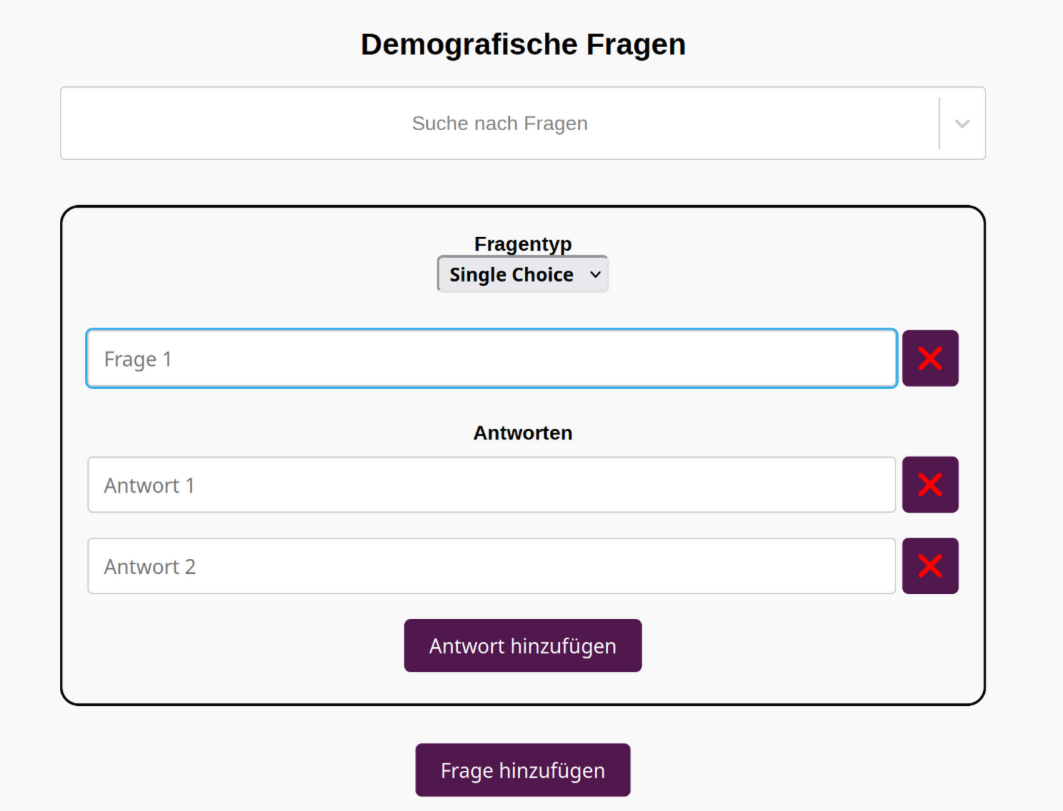
\includegraphics[width=0.6\textwidth]{pics/demographic_question_create.jpg}
	\caption{Create Demographic Question}
	\label{fig:create_dem_que}
\end{figure}
\paragraph{}
The new part for this feature is the search bar. For this the "Select" component of "react-select" is used. The components' controllable state props and modular architecture allows  "isMulti" to select multiple options or "isSearchable" to search. These features, allow easy implementation and an already styled search bar in the project. \parencite{reactselect}
\paragraph{}
The database structure for the demographic questions is similar to the standard ones. The table "PublicQuestions" is used to store the question specific data like name and type. To enable the reuse of questions on different polls "PublicQuestions" is in an many-to-many relationship with "Polls" through "PublicPollQuestions". Answers are stored within the table "PublicAnswers", which is connected to "PublicQuestions" via "PublicQuestionAnswers. This relation is also many-to-many since the options yes or no for example would be used in multiple questions. 
\paragraph{}
For the select every existing question with its answers is fetched from the database and stored within an array. The options are then mapped with the value being id and the label as name of each element. To display the selected options they are mapped through and use the same functions as the standard ones used for the poll. When saving these questions a problem arises, as the selected ones are already stored in the database and possibly changed. To handle this an findOrCreate \ref{fig:publicQuestions} is used to get the existing questions and answers or create new ones. This function also returns each instance found or the created one. With this the question and answer ids can be used for the many-to-many relationship. \parencite{sequelizedoku} 
\begin{figure}[h!]
\begin{code}
let [createdQuestion, created] = await PublicQuestions.findOrCreate({
	where: {
		name: question.name,
		typeId: questionType.id,
	}
});
\end{code}
	\caption{findOrCreate PublicQuestions}
	\label{fig:publicQuestions}
\end{figure}

\section{Edit Polls}
\section{Voting}
\subsection{Disclosed Voting}
\subsection{Anonymous Voting}
\subsection{Public Voting}
The public voting allows users without an account to vote. With this feature a wide range of people can be questioned via street surveys or through a shared link. This poll type has two section, the normal and demographic questions. The order of these play a major role. \textcite{demographicdata} mentions trust, benefits of the demographic data and the ability to abstain. All of these factors have to be taken into ones account when creating these questions. The article also mentions, that at the beginning of a survey the motivation is high and the demographic data are answered, but the trust in full anonymity is decreased. Therefore the author states it is best to put these questions at the end. 
\subsubsection{Vote integrity}
A major problem when having anonymity and no accounts is the data integrity. Without the ability to store information about a voter in the database to check for multiple votes, it is important to prevent them from voting multiple times.  

what to write about:
how to prevent multiple votes: 
- 	captcha against bots 
-	cookies to prevent non techie users 
-	users with knowledge almost impossible to prevent without storing ip or device fingerprints, 
problem with ip and device fp is probably legal reasons

-	userData: which information is important for polls (gender, age, job, )

\section{Results}
\subsection{CSV-Export}
To allow for the further analysis and documentation of the poll results, a CSV export functionality was implemented. This export privides a structured overview of all user responses, including additional metrics such as the number of votes per answer and the average weight for weighted questions.\\ \\
The logic is handled in the \textbf{csvExportController.js} controller. Upon receiving a request, the system retrieves all relevant data for a given poll by its ID, including associated question, answers, and question types. The raw voting data is processed to count the number of responses per answer and to calculate the average weight if applicable. Special care is taken to distinguish between different types: for instance, "Single Choice" questions ensure that only one answer per user is counted, while "Weighted Choice" questions include the weight vale in the computation.\\ \\
The processed data is then converted into a structured CSV format using the json2csv library. The final file includes columns such as Poll Name, Question, Question Type, Answer, Vote Count and Average Weight, and can be downloaded directly by the user. This feature ensures transparency and enables further statistical evaluation using external tools like Excel.\parencite{json2csv}
\section{MyPolls}
\subsection{Polllink}
% Polllink beschreibung von Prasser

To make sharing of the Surveys easier, a QR code generation was implemented. This was done using the React component "qrcode.react" which requires the link to the poll.\parencite{qrcode}
\subsection{Delete Polls}
The deletion of polls is crucial for two main reasons: first, to ensure that all associated data of a survey can be safely removed when necessary and second, to determine when a poll is still eligible for deletion. In this case, the deletion of polls is strictly limited to those that have not yet received any user votes. \\ \\
This constraint ensures the integrity of the data and avoids loss of user-generated information, which could distort statistical analysis or transparency within the system.\\ \\
To maintain data consistency, the deletion process is implemented as a transaction. This guarantees atomicity, meaning that either all steps of the deletion process succeed or none do - preventing partial data deletion and potential corruption. Sequelize's transaction management is used here to wrap the entire process in a rollback-safe structure. \parencite{sequelizedoku}

\paragraph{}
The deletion logic performs the following steps
\begin{enumerate}
	\item Validate that the poll exists.
	\item Fetch all related questions and their IDs.
	\item Check if any user answers exist for these questions. If so abort the operation with an error.
	\item Remove the many-to-many relations between answers from the "QuestionAnswers" table.
	\item Delete the associated answers.
	\item Delete the questions.
	\item Delete any group relations in the "PollGroups" table.
	\item Finally, delete the poll itself.
\end{enumerate}

\begin{figure}[h!]
\begin{code}
	const deletePoll = async (pollId) => {
		const transaction = await sequelize.transaction();
		try {
			...
			await PollGroups.destroy({
				where: { pollId },
				transaction,
			});
			await Polls.destroy({
				where: { id: pollId },
				transaction,
			});
			await transaction.commit();
			return { pollId, questionsDeleted: questionIds.length };
		} catch (error) {
			await transaction.rollback();
			throw error;
		}
\end{code}
\caption{Example for a Sequelize transaction}
\label{fig:delete_poll_code}
\end{figure}
Using Sequelize’s transaction mechanism not only helps to avoid data inconsistency, but also ensures that no information is accidentally deleted once users have participated in a poll. This feature is particularly important in environments where transparency and trust are key, such as in political or organizational voting systems.


\section{Accessibility}
\subsection{Tooltips}
\subsection{Screenreader}
\section{Styling}
\subsection{Generel styling}
The styling of the application was done later in the making process, because only then it was demanded by the customers. The same applies to the color scheme which has two main colors: Yellow and Purple. \\ \\
To ensure consistency of the palette user defined characteristics from CSS where used to assign variables for each main color. \parencite{csscolorvariables}
\begin{figure}[h!]
	\begin{csscode}
		:root {
			--primary-color: #51184e;
			--secondary-color: #F9BB03;
			--primary-hover-color: rgb(163, 131, 168);
		}
	\end{csscode}
	\caption{Variables of the main colors}
	\label{fig:user_defined_characteristics}
\end{figure}

Those variables where then used in each element of where it was needed. Therefore changing the color scheme to a different one is less afford for the end user.

The basic structure of the page is split into three sections: header with navigation, main with content and footer with imprint and privacy policy. The style is based on the client's homepage therefore the standard background is purple but of the content it still is white to ensure readability. \parencite{lmppage}

\subsection{Responsive design}
Responsive design is essential nowadays because users access websites from a wide variety of devices - phones, tablets, laptops and desktops - each with different screen sizes and resolutions. It ensures a seamless, user-friendly experience across all platforms, which improve engagement and accessibility.\\ \\
To ensure responsiveness in each section of the application, "@media CSS at-rule" was used to apply different styles based on the screen size or device characteristics. This approach allows the layout, font sizes and element spacing to adapt dynamically, creating a smoother experience for users on any device. The navigation bar was designed with media queries to transform into so-called "burger menu" when the screen width falls below a certain threshold. This ensures usability on smaller devices like smartphones because the elements within the navigation get displayed in the menu now.
\begin{figure}[h!]
	\centering
	
\includegraphics[width=1\textwidth]{pics/navigation.png}
	\caption{Navigation}
	\label{fig:navigation}
\end{figure}
\begin{figure}[H]
	\centering
	
\includegraphics[width=0.3\textwidth]{pics/burger_menu.png}
	\caption{Burger menu}
	\label{fig:burger_menu}
\end{figure}
\subsection{Individual styling}

\chapter{Summary}
\lipsum[1]

% Literaturverweis-Beispiel
Hier ein Zitat aus einer Quelle \cite{author2023example}.

% Zusammenfassung


% Literaturverzeichnis
\printbibliography

% Abbildungsverzeichnis
\listoffigures
\newpage

\end{document}
